% !TEX program = pdflatex
% -----------------------------------------------------------------------------
% EgoBrain IRIS Manuscript
% Springer Computer Science proceedings / LNEE-compatible LLNCS manuscript.
% Figures and tables are expected in ./figures/ and ./tables/.
% -----------------------------------------------------------------------------

\documentclass[runningheads]{llncs}

\usepackage[T1]{fontenc}
\usepackage{newtxtext}
\usepackage[varvw]{newtxmath}
\usepackage{graphicx}
\usepackage{booktabs}
\usepackage{url}

\begin{document}

\title{NeuroRoute: Neural-Temporal Supervision for Adaptive Computation in Egocentric Video Recognition}

\titlerunning{NeuroRoute for Egocentric Video Recognition}

\author{
Keerthi Kumar K. J.\inst{1}\and
Razeena Tasneem B.\inst{2}\and
Naveena R.\inst{2}\and
Abdul Arshath S.\inst{3}\and
Maheswar R.\inst{1}}

\authorrunning{K. K. J. Keerthi et al.}

\institute{
Department of Electronics and Communication Engineering, KPR Institute of Engineering and Technology, Coimbatore, India\\
\email{REPLACE-WITH-CORRESPONDING-AUTHOR-EMAIL}
\and
Department of Computer Science and Engineering, KPR Institute of Engineering and Technology, Coimbatore, India
\and
Department of Information Technology, KPR Institute of Engineering and Technology, Coimbatore, India
}

\maketitle

\begin{abstract}
Egocentric action recognition requires temporal reasoning over sequential visual evidence, yet dense temporal processing can be redundant and costly, while practical streams may contain missing or corrupted observations. This work investigates whether synchronized electroencephalography (EEG) can serve as training-time privileged information for learning how a visual model allocates temporal computation, while retaining video-only inference. We construct a subject-independent benchmark from 40 EgoBrain participants using a rigorously synchronized one-second index, yielding 227,864 synchronized temporal records and a fixed 27-class evaluation protocol with 24/8/8 subject splits. A standalone EEG temporal teacher achieves a test macro-F1 of 0.03888 against the $1/27=0.03704$ reference, but temporal-shuffle degradation is only 0.00088 and normalized temporal-importance entropy is 0.99978, indicating limited evidence for a strongly concentrated neural temporal prior. We then reproduce an adaptive temporal-routing pipeline under explicit token budgets. At the predefined 50\% budget, temporal computation falls from 35,927,552 to 17,905,152 estimated FLOPs per sample, a 50.16\% reduction, and deployment requires neither EEG preprocessing nor an EEG encoder. However, the deployed route does not preserve recognition (macro-F1 0.03483 vs. 0.03753 for the dense visual reference) or improve mean corruption robustness (0.03293 vs. 0.03530). The study therefore establishes a reproducible neural-supervision and adaptive-computation framework, while also identifying the current limits of transferring weak EEG temporal structure into visual inference.

\keywords{Egocentric video \and action recognition \and EEG \and privileged information \and temporal routing \and adaptive computation \and multimodal learning}
\end{abstract}

% =============================================================================
\section{Introduction}
% =============================================================================

Egocentric vision studies visual perception from a first-person viewpoint and is increasingly used to model human--object interaction, daily activities, and long-horizon behavior. Large-scale resources such as EPIC-KITCHENS and Ego4D established the importance of temporal context, environmental diversity, and subject variability in first-person video understanding~\cite{damen2022epickitchens,grauman2022ego4d}. Temporal modeling is consequently central to action recognition: the relevant evidence is rarely contained in an isolated frame and can instead be distributed over an interval of motion, object interaction, and context.

Transformer-based video models provide a natural mechanism for temporal reasoning~\cite{bertasius2021timesformer,arnab2021vivit,tong2022videomae}. At the same time, the same temporal redundancy that helps recognition can create an efficiency problem. Adaptive video systems have therefore explored selective processing, early exiting, spatially focused computation, and token sparsification~\cite{wang2021adafocus,ghodrati2021frameexit,ryoo2021tokenlearner,rao2021dynamicvit,wang2022adafocusv2}. More recent work continues to study temporal compression and token reduction for large-scale video and multimodal systems~\cite{fu2025framefusion,li2026adaptok}.

A complementary source of information is human neural activity. EgoBrain introduced a large-scale dataset synchronizing first-person video and EEG over extended periods, with 40 participants and 29 daily-activity categories, and its authors proposed Brain-TIM for multimodal action understanding~\cite{lin2026egobrain}. Prior work has also shown that EEG can be used as privileged information for video-based action understanding, with the auxiliary neural modality removed at inference time~\cite{cavazza2022actions}. More broadly, learning using privileged information formalizes the use of training-time information that is unavailable during deployment~\cite{vapnik2009privileged}, while knowledge distillation provides a general teacher--student mechanism for transferring information between models~\cite{hinton2015distillation}.

The central question considered here is narrower and more computationally oriented: \emph{can temporally synchronized neural dynamics be used not merely to improve multimodal prediction, but to supervise which temporal evidence a visual model should retain?} This reframes EEG as a training-time temporal prior for adaptive visual computation rather than as an inference-time modality. The resulting architecture is asymmetric: EEG is available to the teacher during training, while the deployed system receives video alone.

The work makes three contributions. First, we establish a reproducible, subject-independent EgoBrain evaluation pipeline with explicit temporal alignment, semantic label construction, leakage controls, and a frozen evaluation split. Second, we provide a controlled EEG-teacher analysis that quantifies how much action-discriminative and temporally ordered information is present in the extracted neural representation. Third, we evaluate an EEG-supervised adaptive temporal-routing mechanism under explicit compute budgets, including temporal corruption tests, neural negative controls, subject-level paired analysis, and an EEG-free deployment audit. Importantly, the study reports both the positive efficiency result and the negative recognition/robustness findings rather than treating an inconclusive routing experiment as a performance improvement.

% =============================================================================
\section{Related Work}
% =============================================================================

\subsection{Egocentric action recognition and temporal modeling}

First-person datasets expose action recognition to viewpoint-dependent appearance, long temporal context, repeated activities, and subject variation. EPIC-KITCHENS-100 provides long-form first-person recordings with dense action annotations~\cite{damen2022epickitchens}, while Ego4D broadened the problem to thousands of hours and diverse daily-life settings~\cite{grauman2022ego4d}. Modern video transformers such as TimeSformer and ViViT model spatiotemporal dependencies using self-attention~\cite{bertasius2021timesformer,arnab2021vivit}; VideoMAE further demonstrated the effectiveness of masked video pre-training for learning compact video representations~\cite{tong2022videomae}. These methods motivate the dense temporal visual backbone used as the reference model in this study.

\subsection{EEG and neural signals for visual understanding}

The EgoBrain benchmark explicitly couples first-person video with EEG and evaluates cross-subject and cross-environment action understanding~\cite{lin2026egobrain}. The dataset authors use modality-specific feature extraction followed by multimodal temporal modeling, establishing EEG--vision fusion as a strong baseline paradigm. In a different setting, Cavazza et al. used EEG responses elicited by action videos as privileged information for video classification and trained models that could be deployed with video alone~\cite{cavazza2022actions}. These results motivate the asymmetric teacher--student setting adopted here, but our focus is different: rather than treating EEG primarily as a source of additional class evidence, we test whether its temporal structure can supervise \emph{where visual computation should be allocated}.

\subsection{Privileged information and knowledge transfer}

Learning Using Privileged Information (LUPI) formalizes learning systems that exploit additional information available during training but absent during deployment~\cite{vapnik2009privileged}. Knowledge distillation provides a practical teacher--student mechanism for transferring predictive structure or intermediate representations~\cite{hinton2015distillation}. Our formulation follows this asymmetric logic but applies it to temporal computation: the neural teacher is used only during training, and the visual student is ultimately required to operate without EEG.

\subsection{Adaptive computation for video}

Efficient video recognition has been approached using adaptive spatial attention, conditional early exiting, learned token selection, and dynamic token sparsification. AdaFocus identifies informative spatial regions and can also incorporate temporal frame skipping~\cite{wang2021adafocus}; FrameExit dynamically changes the amount of processed video based on input difficulty~\cite{ghodrati2021frameexit}. TokenLearner learns a small set of adaptive tokens for image and video processing~\cite{ryoo2021tokenlearner}, while DynamicViT demonstrates differentiable dynamic token sparsification~\cite{rao2021dynamicvit}. AdaFocus V2 further explores efficient end-to-end training and adaptive temporal computation~\cite{wang2022adafocusv2}. Recent video-token work continues to reduce temporal and visual redundancy through similarity-aware token reduction and content-dependent allocation~\cite{fu2025framefusion,li2026adaptok}. These methods establish adaptive temporal computation as an active computer-vision problem; our study asks whether neural activity can provide a privileged supervisory signal for the routing decision.

\subsection{Temporal corruption and robustness}

Temporal corruption can invalidate assumptions made by dense sequence models. Zeng et al. introduced dedicated temporal-corruption benchmarks and showed that video temporal-analysis systems can be highly sensitive even to limited corruption~\cite{zeng2024temporalrobustness}. Motivated by this line of work, we evaluate six controlled temporal corruption families across multiple severities. Robustness is treated as an evaluation axis rather than being assumed to arise from adaptive routing.

% =============================================================================
\section{Dataset, Synchronization, and Problem Formulation}
% =============================================================================

\subsection{EgoBrain and synchronized modalities}

EgoBrain provides synchronized first-person video and EEG from 40 participants performing daily activities~\cite{lin2026egobrain}. The dataset is naturally suited to studying whether external visual evidence and internal neural dynamics can be related on a shared timeline. The published EgoBrain benchmark uses its own multimodal protocol and reports results for both cross-subject and cross-environment settings. The present study does not attempt to reproduce those published scores directly; instead, it defines a frozen feature-level benchmark whose purpose is to isolate the temporal-supervision question under a common subject-independent split.

\subsection{Temporal feature representation}

For each temporal step $t$, the visual stream is represented by a precomputed feature vector
$\mathbf{x}^{V}_{t}\in\mathbb{R}^{512}$ and the EEG stream by
$\mathbf{x}^{E}_{t}\in\mathbb{R}^{128}$. The EEG representation is sampled at 256~Hz before temporal feature aggregation. We use an 8-step sequence with one-second temporal units, so a training example is written as
\begin{equation}
\mathbf{X}^{V}=\{\mathbf{x}^{V}_{1},\ldots,\mathbf{x}^{V}_{8}\},
\qquad
\mathbf{X}^{E}=\{\mathbf{x}^{E}_{1},\ldots,\mathbf{x}^{E}_{8}\}.
\end{equation}

\subsection{Temporal synchronization and label construction}

The data-processing pipeline constructs an explicit one-second synchronized index rather than assuming that feature-row order alone implies temporal alignment. The locked record contains 227,864 synchronized one-second rows across 40 participants. Twenty-nine retained canonical/lifecycle categories are preserved in the alignment artifacts, while the downstream classifier uses 27 semantic action classes. Lifecycle/system events are excluded from the same-label eight-second classification windows because they do not define stable semantic action intervals.

\subsection{Subject-independent evaluation}

To prevent temporal-window leakage across participants, the primary split is subject-disjoint: 24 participants for training, 8 for validation, and 8 for testing. The resulting sequence counts are 31,147, 38,404, and 46,178, respectively. All model selection decisions are made using validation data only; the test set is reserved for the final reported comparison.

\subsection{Integrity and leakage controls}

The synchronization stage includes visual and EEG timeline audits, marker-clock checks, boundary validation, cross-modal overlap checks, and subject-level alignment records. The final locked artifacts preserve the mapping from synchronized temporal rows to the corresponding visual and EEG indices. The resulting evaluation therefore isolates model behavior from common errors caused by random window splitting, subject overlap, or implicit temporal misalignment.

{\small\begin{table}[t]
\centering
\caption{EgoBrain scale and frozen subject-independent evaluation split.}
\label{tab:dataset}
\begin{tabular}{lrr}
\toprule
Split & Subjects & Sequences \\
\midrule
Train & 24 & 31147 \\
Val & 8 & 38404 \\
Test & 8 & 46178 \\
Total / source & 40 & 227,864 synchronized rows \\
\bottomrule
\end{tabular}
\par\smallskip\noindent\footnotesize\textit{Note.} The 27-class classifier uses semantic action labels; lifecycle markers are retained for audit but excluded from same-label 8-s windows.
\end{table}
}

% =============================================================================
\section{Neural-Temporal Supervision and Adaptive Routing}
% =============================================================================

\subsection{Visual temporal backbone}

The visual reference model is a temporal Transformer operating on the 8-step, 512-dimensional feature sequence. The dense backbone is intentionally kept fixed across the downstream experiments so that any change in recognition or compute is attributable to the temporal supervision and routing mechanism rather than to a changing feature extractor. The frozen visual benchmark contains simple pooling, temporal convolution, temporal Transformer, and masked temporal Transformer references; the temporal Transformer provides the primary dense backbone for the routing study.

Let
\begin{equation}
\mathbf{z}^{V}_{t}=f_{V}(\mathbf{x}^{V}_{1:8})_{t}
\end{equation}
be the temporal visual representation at step $t$.

\subsection{EEG temporal teacher}

The EEG teacher receives the aligned sequence $\mathbf{X}^{E}$ and learns a temporal representation
\begin{equation}
\mathbf{z}^{E}_{t}=f_{E}(\mathbf{x}^{E}_{1:8})_{t}.
\end{equation}
A classification head provides an independent estimate of whether the neural representation contains action-discriminative information. In addition, the teacher produces normalized temporal-importance scores $\mathbf{a}^{E}\in\mathbb{R}^{8}$.

The teacher is evaluated independently before it is used as a supervisory source. This step is essential because privileged information is only useful when the teacher signal contains reliable information relevant to the target problem.

\subsection{Neural temporal-relation supervision}

Rather than imposing a direct pointwise mapping between the 128-dimensional EEG representation and the 512-dimensional visual representation, we compare their temporal geometry. For a sequence, define pairwise relation matrices
\begin{equation}
R^{E}_{ij}=d(\mathbf{z}^{E}_{i},\mathbf{z}^{E}_{j}),
\qquad
R^{V}_{ij}=d(\mathbf{z}^{V}_{i},\mathbf{z}^{V}_{j}),
\end{equation}
where $d(\cdot,\cdot)$ denotes a normalized distance. A relation-transfer objective can then be written as
\begin{equation}
\mathcal{L}_{\mathrm{rel}}
=
\frac{1}{T^{2}}\sum_{i,j}
\left|R^{V}_{ij}-R^{E}_{ij}\right|.
\end{equation}

The intention is not to claim that neural and visual features occupy the same semantic space. Instead, the student is encouraged to preserve useful aspects of the teacher's temporal organization.

\subsection{Temporal-importance supervision}

The teacher's temporal-importance distribution is compared with the visual router distribution. Let $\mathbf{a}^{V}$ denote the normalized visual importance scores. The corresponding supervision term is
\begin{equation}
\mathcal{L}_{\mathrm{imp}}
=
D_{\mathrm{KL}}
\left(\mathbf{a}^{E}\;\|\;\mathbf{a}^{V}\right).
\end{equation}
This term explicitly connects neural temporal evidence to the later keep/drop decision.

\subsection{Adaptive temporal router}

The router maps each visual temporal representation to a scalar score:
\begin{equation}
s_{t}=g(\mathbf{z}^{V}_{t}),
\qquad
\mathbf{a}^{V}=\mathrm{softmax}(\mathbf{s}).
\end{equation}
For a target retention fraction $\rho$, the router keeps
\begin{equation}
k=\max(1,\lfloor\rho T\rfloor)
\end{equation}
temporal tokens with the highest scores. Since $T=8$, the principal 50\% budget retains $k=4$ temporal tokens.

\subsection{Budget-aware objective}

The downstream objective combines semantic recognition, neural relation transfer, temporal-importance supervision, robustness, and a budget term:
\begin{equation}
\mathcal{L}
=
\mathcal{L}_{\mathrm{cls}}
+\lambda_{r}\mathcal{L}_{\mathrm{rel}}
+\lambda_{i}\mathcal{L}_{\mathrm{imp}}
+\lambda_{b}\mathcal{L}_{\mathrm{budget}}
+\lambda_{c}\mathcal{L}_{\mathrm{robust}}.
\end{equation}
The terms are activated sequentially during the development pipeline so that the contribution of each component can be assessed rather than introducing an unconstrained collection of losses simultaneously.

\subsection{Training-only neural supervision and deployment}

The key deployment property is asymmetric modality availability. During training, the EEG teacher supplies auxiliary information to the visual branch. During inference, the teacher and EEG input are removed:
\begin{equation}
\text{Video}\rightarrow\text{Visual Encoder}\rightarrow\text{Temporal Router}\rightarrow\text{Action}.
\end{equation}
No EEG preprocessing, EEG encoder, or neural inference branch is required at deployment. This makes the deployed system a conventional video-only predictor with a training-time privileged signal.

\begin{figure}[t]
\centering
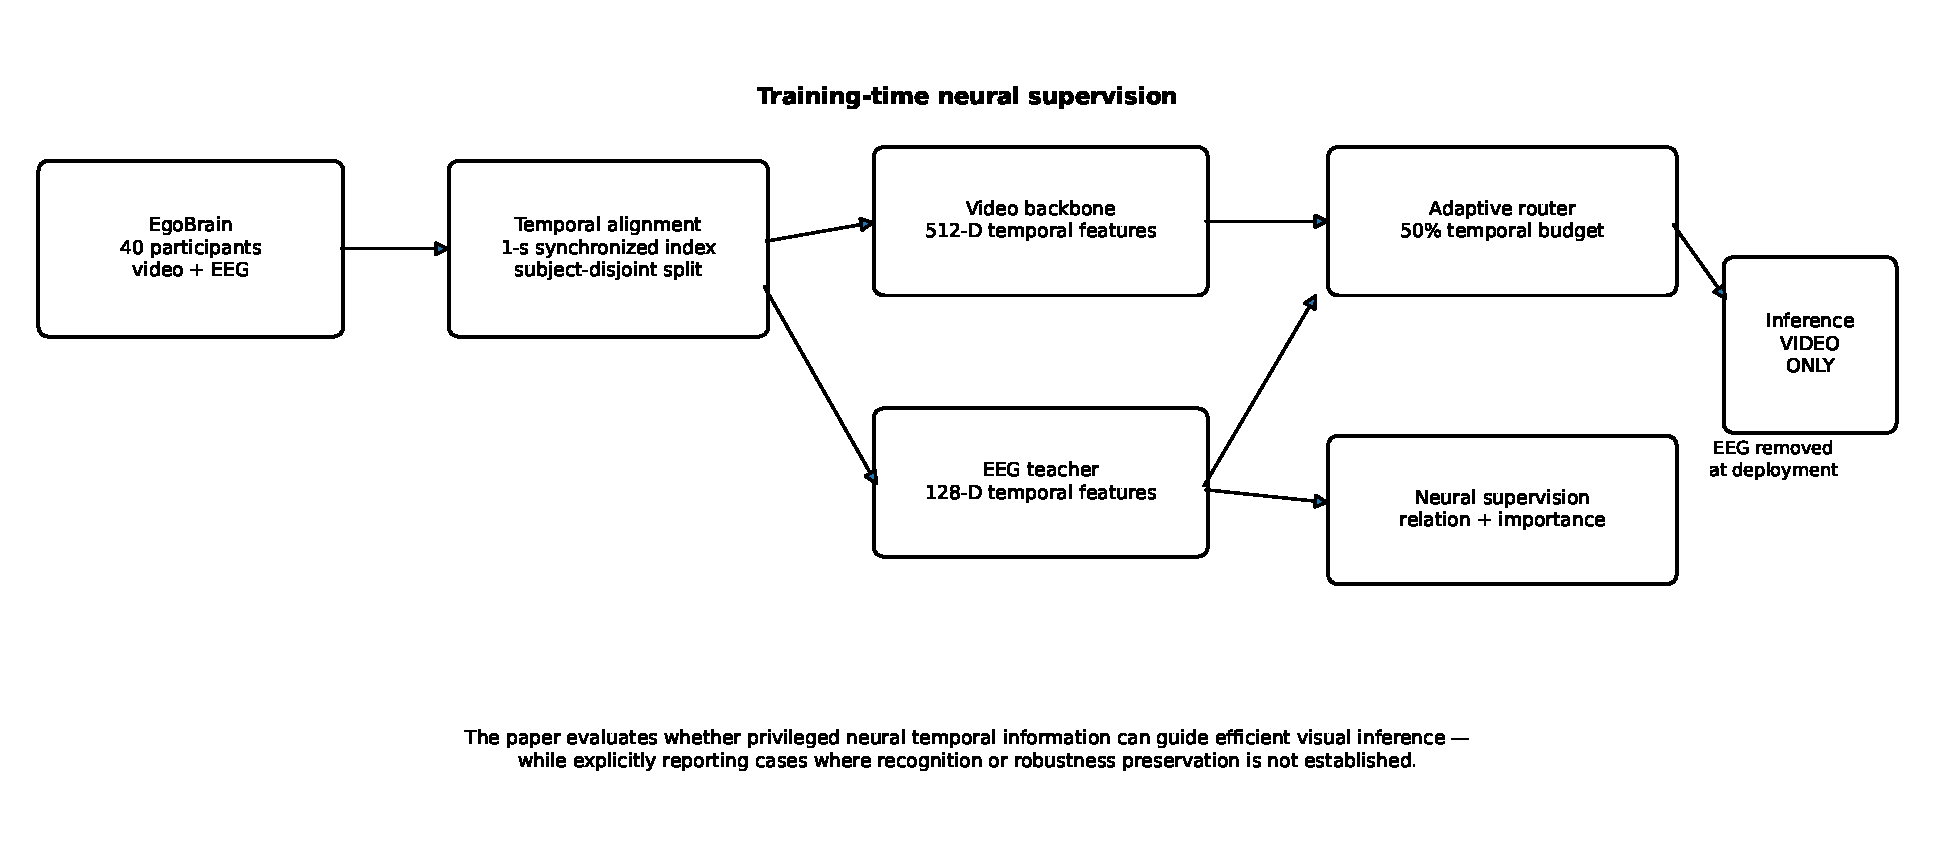
\includegraphics[width=\linewidth]{figures/fig01_study_framework.pdf}
\caption{Overview of the study and NeuroRoute training/deployment asymmetry. EEG is used as training-time privileged information and is removed completely from the deployed visual inference path.}
\label{fig:framework}
\end{figure}

% =============================================================================
\section{Experimental Protocol}
% =============================================================================

\subsection{Metrics and evaluation principles}

We report accuracy, balanced accuracy, macro-F1, and weighted F1. Macro-F1 is the primary comparison because the action distribution is non-uniform and the objective is to evaluate performance across the full 27-class label space rather than allow dominant classes to determine the aggregate score. The reference chance macro-F1 is taken as $1/27=0.03704$.

\subsection{Video-only baseline ladder}

The visual benchmark compares mean pooling, max pooling, mean+max pooling, temporal convolution, temporal Transformer, and masked temporal Transformer. Parameter count, estimated forward FLOPs per sample, and inference latency are recorded alongside the recognition metrics. The temporal Transformer is selected as the primary dense reference using validation-only model selection.

\subsection{Temporal corruption benchmark}

The robustness protocol applies six corruption families: random frame/clip dropping, burst deletion, temporal jitter, irregular sampling, playback-speed change, and contiguous temporal blackout. Each corruption is evaluated at severities 0.05, 0.15, 0.30, 0.50, and 0.70. These perturbations are applied as controlled evaluation conditions; the corruption protocol is fixed before the final comparison.

\subsection{Temporal compute budgets}

The routing study evaluates retention budgets of 100\%, 75\%, 50\%, 25\%, and 12.5\%. For the main 50\% experiment, four of eight temporal tokens are retained. We report the resulting estimated temporal FLOPs and recognition metrics together, because token count alone does not establish computational benefit.

\subsection{Neural negative controls}

To test whether the downstream result depends on meaningful neural supervision, the completed pipeline includes random EEG, wrong-subject EEG, temporally shifted EEG, and a no-neural-supervision condition. These controls preserve the overall architecture while disrupting the semantic relationship between the visual and neural streams.

\subsection{Subject-level paired analysis}

Aggregate recognition scores can mask heterogeneous behavior across participants. We therefore compare the dense reference and the deployed route on the eight held-out test subjects and report the mean paired macro-F1 difference together with a 95\% bootstrap confidence interval.

% =============================================================================
\section{Results}
% =============================================================================

\subsection{Study scale and evaluation integrity}

The final synchronized index contains 227,864 one-second rows from 40 participants, with a frozen 24/8/8 subject split producing 31,147 training, 38,404 validation, and 46,178 test sequences (Table~\ref{tab:dataset}). This locked split is reused throughout the visual baseline, EEG-teacher, and routing studies. Figure~\ref{fig:dataset} summarizes the scale of the temporal records and subject-independent evaluation subsets.

\begin{figure}[t]
\centering
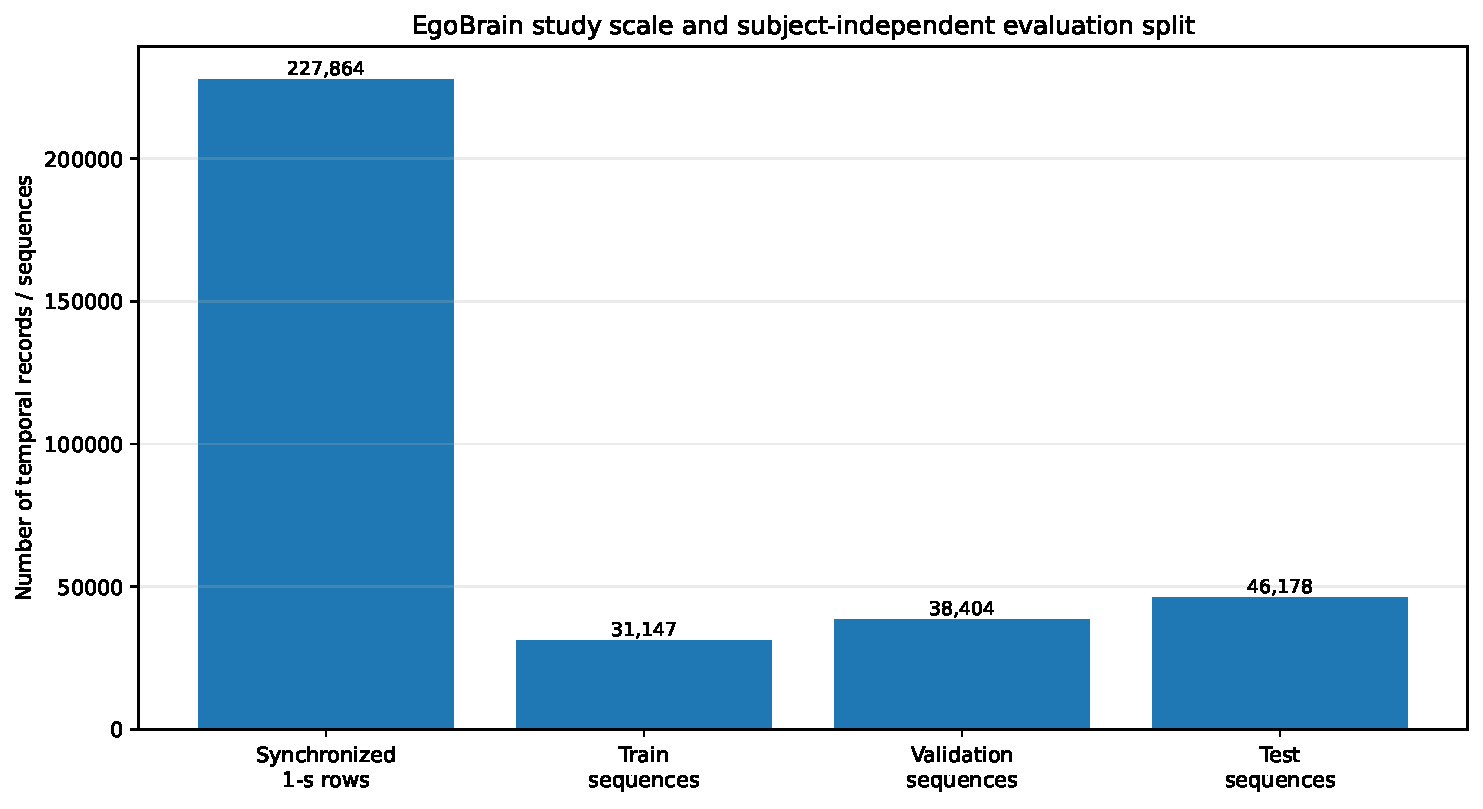
\includegraphics[width=0.92\linewidth]{figures/fig02_dataset_and_split.pdf}
\caption{Scale of the synchronized EgoBrain index and the frozen subject-independent evaluation split.}
\label{fig:dataset}
\end{figure}

\subsection{Video-only baseline establishes a difficult reference}

The primary dense visual reference achieves a clean test accuracy of approximately 0.05143, balanced accuracy of approximately 0.03969, macro-F1 of 0.03753, and weighted F1 of 0.04918. The macro-F1 is only modestly above the $1/27$ reference, indicating that the subject-independent 27-class feature-level problem is difficult under the locked protocol. This result is important for interpreting every downstream gain or loss: an adaptive model should not be described as successful merely because it reduces compute if recognition is simultaneously degraded.

Table~\ref{tab:vision_baselines} contains the full frozen baseline ladder, including parameter count and estimated computation. Figure~\ref{fig:baselines} visualizes the same comparison relative to the 27-class reference level.

{\scriptsize\begin{table}[t]
\centering
\caption{Clean test performance of the frozen video-only baseline ladder.}
\label{tab:vision_baselines}
\begin{tabular}{lrrrrrrr}
\toprule
Model & Accuracy & Balanced Acc. & Macro-F1 & Weighted F1 & Params & FLOPs/sample & Latency (ms) \\
\midrule
Mean pool & 0.0314 & 0.0288 & 0.0252 & 0.0289 & 13851 & 31744 & 0.0003 \\
Max pool & 0.0405 & 0.0331 & 0.0323 & 0.0388 & 13851 & 31744 & 0.0004 \\
Mean + max & 0.0398 & 0.0350 & 0.0307 & 0.0359 & 27675 & 63488 & 0.0006 \\
Temporal conv & 0.0391 & 0.0359 & 0.0317 & 0.0378 & 326043 & 5122176 & 0.0055 \\
Temporal Transformer & 0.0514 & 0.0397 & 0.0376 & 0.0492 & 2247195 & 35927552 & 0.0287 \\
Masked Transformer & 0.0382 & 0.0310 & 0.0296 & 0.0358 & 2247195 & 35927552 & 0.0286 \\
\bottomrule
\end{tabular}
\par\smallskip\noindent\footnotesize\textit{Note.} The primary downstream visual backbone is the Temporal Transformer. Chance macro-F1 for 27 classes is 0.03704.
\end{table}
}

\begin{figure}[t]
\centering
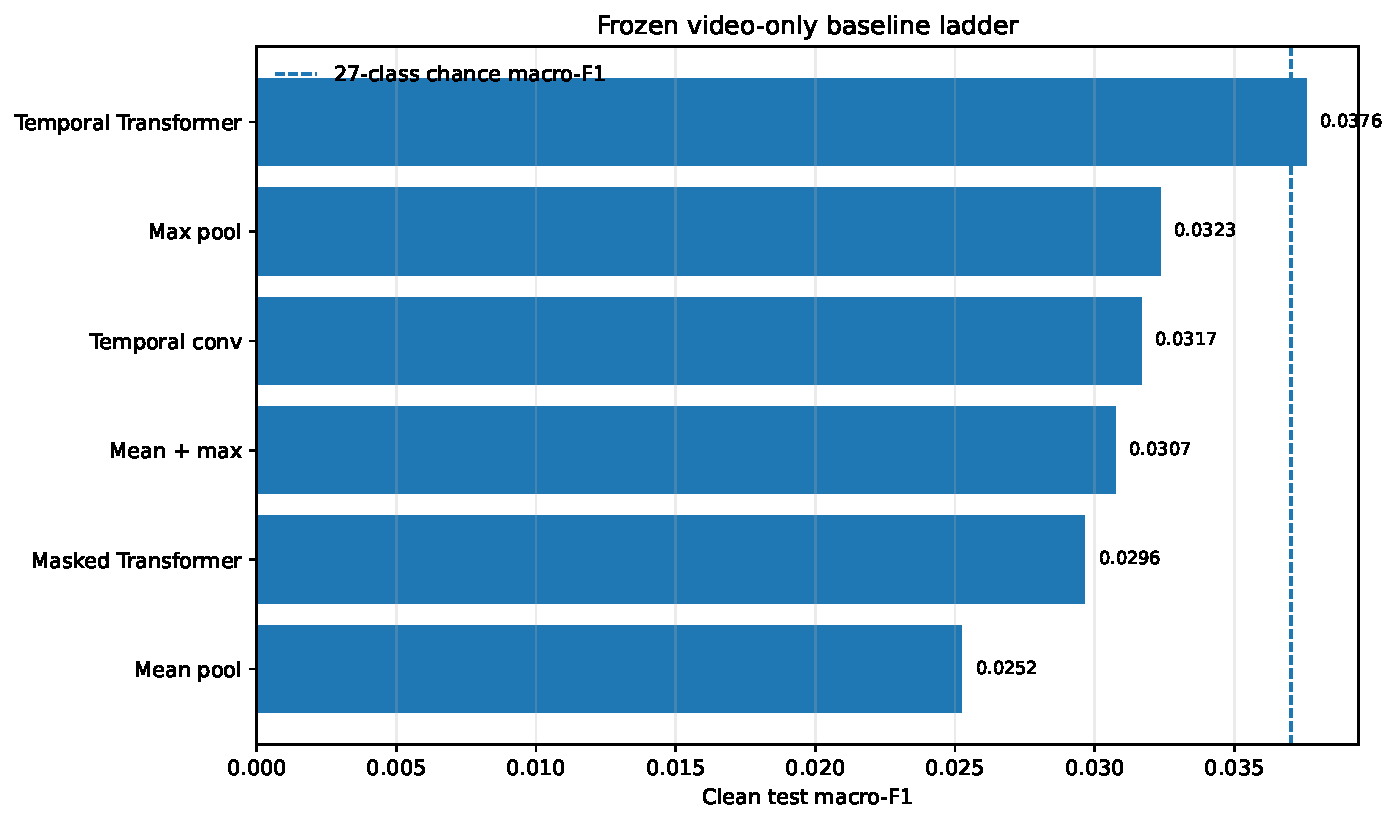
\includegraphics[width=0.92\linewidth]{figures/fig03_visual_baselines.pdf}
\caption{Frozen video-only baseline ladder on the subject-independent test split.}
\label{fig:baselines}
\end{figure}

\subsection{EEG teacher contains weak action-discriminative information}

The later standalone EEG-teacher diagnostic selects a temporal Transformer using validation macro-F1. The selected model obtains 0.04120 validation macro-F1 and 0.03888 test macro-F1, compared with the $1/27=0.03704$ reference (Table~\ref{tab:eeg_teacher}). This difference is small but measurable and motivates testing whether the neural representation can serve as a privileged training signal.

The temporal diagnostics, however, do not indicate a strong or sharply concentrated neural temporal prior. Temporal shuffling decreases test macro-F1 by only 0.00088, while normalized temporal-importance entropy is 0.99978, very close to the uniform eight-step entropy. The mean adjacent-token cosine similarity is 0.99545, further indicating that the extracted temporal representations are highly similar between adjacent steps. The mean held-out-subject macro-F1 is 0.03703. Figure~\ref{fig:eegteacher} summarizes these diagnostics. The combined evidence therefore supports a cautious interpretation: the EEG representation contains weak action-related information, but the current feature representation does not provide strong evidence for highly localized temporal supervision.

{\small\begin{table}[t]
\centering
\caption{Standalone EEG temporal-teacher performance; selected by validation macro-F1 (temporal\textbackslash{}_transformer).}
\label{tab:eeg_teacher}
\begin{tabular}{lrrrr}
\toprule
Split & Accuracy & Balanced Acc. & Macro-F1 & Weighted F1 \\
\midrule
train & 0.0742 & 0.0370 & 0.0051 & 0.0102 \\
val & 0.1066 & 0.0370 & 0.0071 & 0.0205 \\
test & 0.0869 & 0.0370 & 0.0059 & 0.0139 \\
\bottomrule
\end{tabular}
\par\smallskip\noindent\footnotesize\textit{Note.} Chance macro-F1 = 0.03704; temporal-shuffle macro-F1 drop = 0.00088; normalized importance entropy = 0.99978.
\end{table}
}

\begin{figure}[t]
\centering
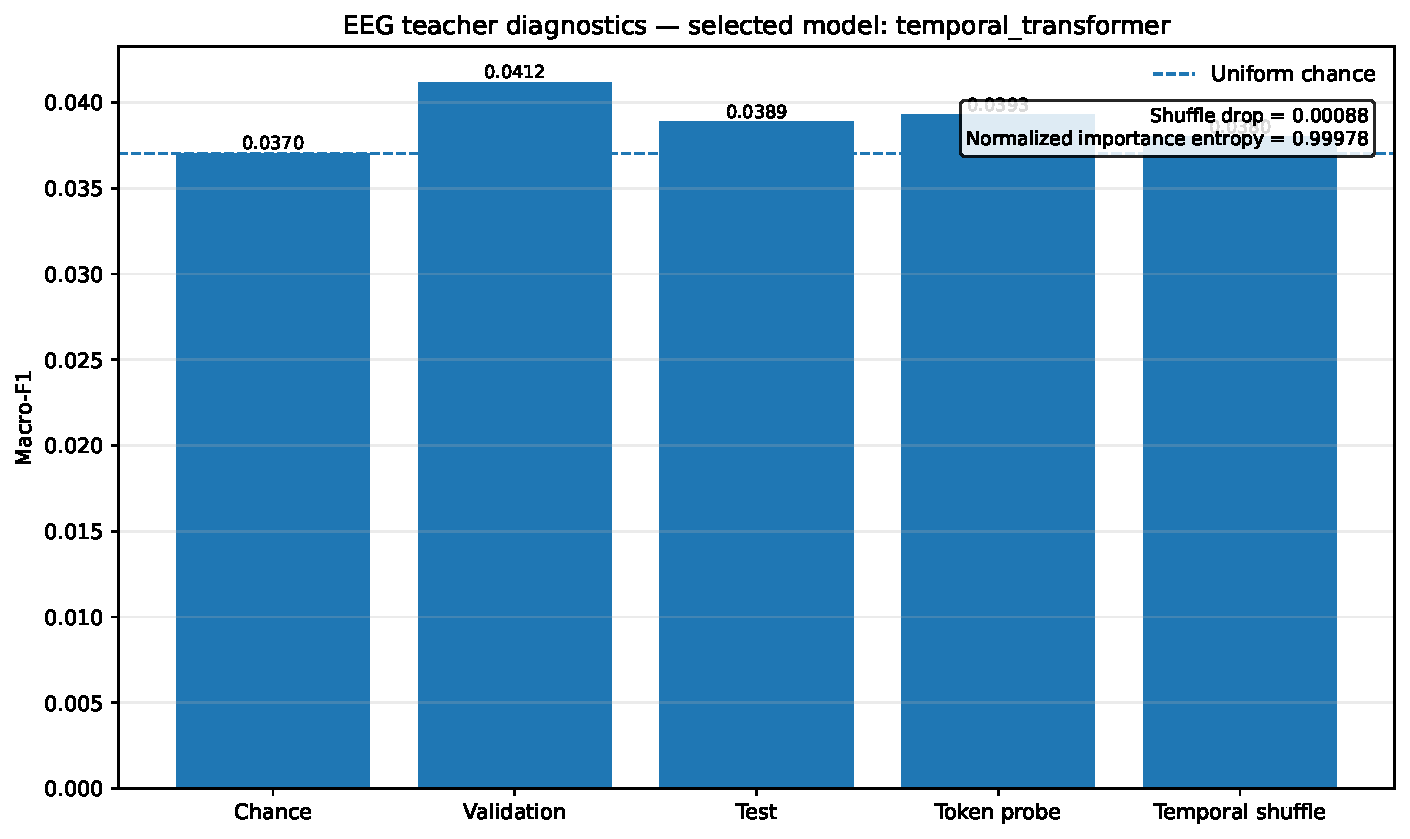
\includegraphics[width=0.92\linewidth]{figures/fig04_eeg_teacher_diagnostics.pdf}
\caption{Standalone EEG-teacher diagnostics. The predictive signal is weak, and the temporal-order and importance-concentration tests provide limited evidence for a strong neural temporal prior.}
\label{fig:eegteacher}
\end{figure}

\subsection{Adaptive routing reduces temporal computation but does not preserve recognition}

At the predefined 50\% retention budget, the routing system processes four of eight temporal tokens. The estimated temporal computation decreases from 35,927,552 FLOPs per sample for the dense reference to 17,905,152 FLOPs per sample for the routed configuration, corresponding to a 50.16\% reduction (Table~\ref{tab:compute_budget}). Figure~\ref{fig:compute} presents the budget--compute relationship together with the recognition measurements available for the completed routing sweep.

This reduction is a concrete positive result, but it must be separated from recognition quality. In the final visual-only deployment audit, NeuroRoute reaches 0.03483 macro-F1 compared with 0.03753 for the dense visual reference. The paired unseen-subject macro-F1 difference is +0.000094 with a 95\% bootstrap interval of $[-0.010227,0.012364]$, which crosses zero. Consequently, the current experiments do not establish recognition preservation under the 50\% budget.

{\small\begin{table}[t]
\centering
\caption{Temporal compute budget sweep and estimated temporal FLOP reduction.}
\label{tab:compute_budget}
\begin{tabular}{lrrrr}
\toprule
Budget & Tokens & Temporal FLOPs & FLOP reduction & Latency (ms) \\
\midrule
100.0\textbackslash{}% & 8 & 35927552 & 0.0000 & 1.8765 \\
75.0\textbackslash{}% & 6 & 26899968 & 0.2513 & 1.9064 \\
50.0\textbackslash{}% & 4 & 17905152 & 0.5016 & 1.6867 \\
25.0\textbackslash{}% & 2 & 8943104 & 0.7511 & 1.6805 \\
12.5\textbackslash{}% & 1 & 4474368 & 0.8755 & 1.8875 \\
\bottomrule
\end{tabular}
\par\smallskip\noindent\footnotesize\textit{Note.} At the predefined 50\textbackslash{}% budget, temporal computation decreases from 35,927,552 to 17,905,152 FLOPs/sample (50.16\textbackslash{}% reduction).
\end{table}
}

\begin{figure}[t]
\centering
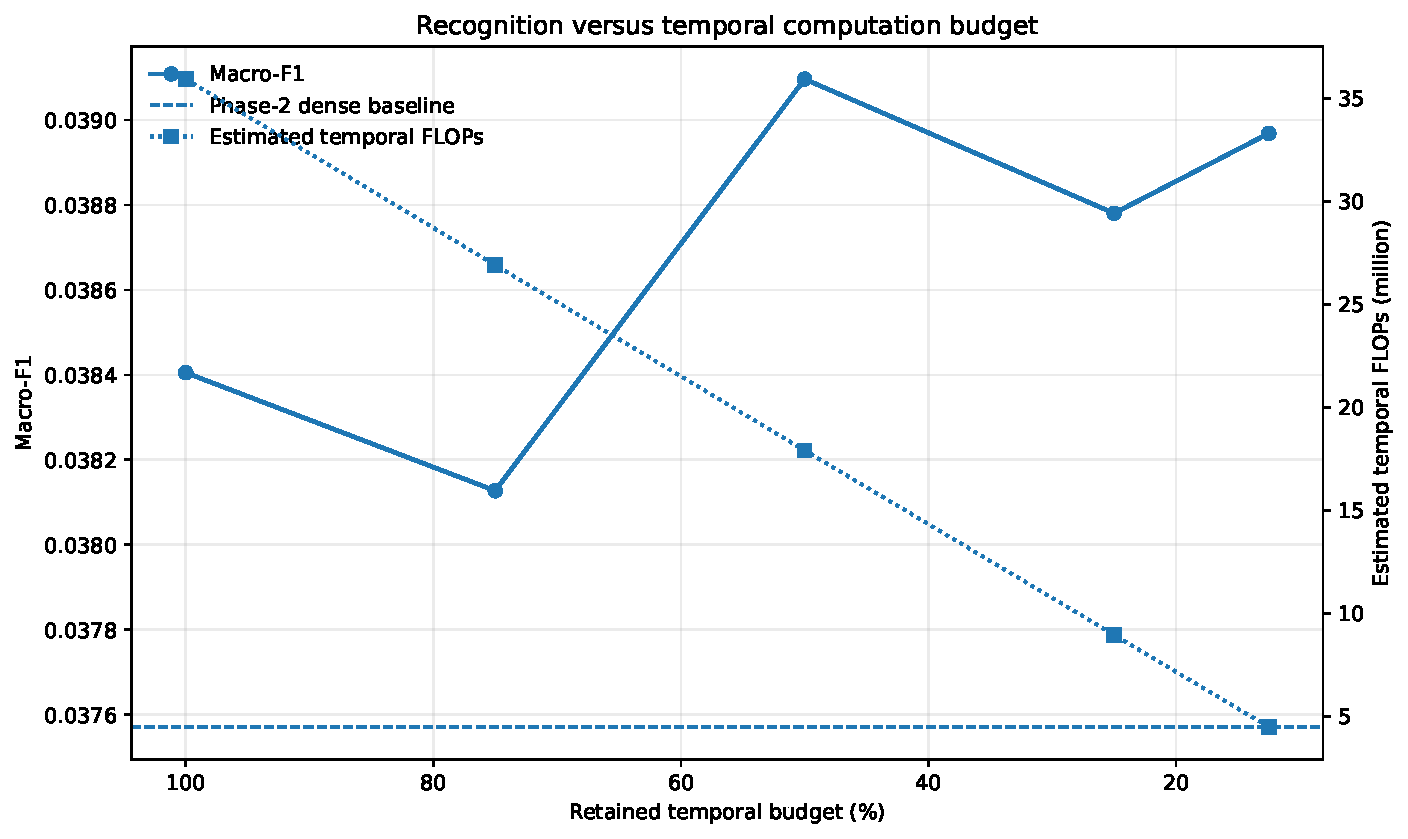
\includegraphics[width=0.92\linewidth]{figures/fig05_compute_budget.pdf}
\caption{Adaptive temporal-computation sweep. The principal 50\% budget retains four of eight temporal tokens and reduces estimated temporal FLOPs by 50.16\%.}
\label{fig:compute}
\end{figure}

\subsection{Temporal corruption robustness is not improved by the completed route}

The dense reference has a mean corruption macro-F1 of 0.03530 across the complete severity grid, whereas the 50\% deployed route reaches 0.03293, yielding a difference of $-0.00237$ (Table~\ref{tab:robustness}). Figure~\ref{fig:robustness} reports the six corruption families and their severity-dependent behavior. The route therefore does not support a claim of improved robustness under the present frozen protocol.

This negative result is informative because it prevents a common confound: an adaptive mechanism can reduce the nominal amount of processed temporal information while simultaneously discarding evidence that remains necessary for recognition under corrupted inputs. The present result shows that computation reduction alone is insufficient evidence of robust adaptive inference.

{\small\begin{table}[t]
\centering
\caption{Temporal-corruption robustness comparison for the dense visual baseline and 50\textbackslash{}% NeuroRoute deployment.}
\label{tab:robustness}
\begin{tabular}{lrrr}
\toprule
Corruption & Phase-2 F1 & NeuroRoute F1 & Δ F1 \\
\midrule
burst deletion & 0.0318 & 0.0243 & -0.0074 \\
contiguous blackout & 0.0360 & 0.0254 & -0.0106 \\
irregular sampling & 0.0375 & 0.0352 & -0.0022 \\
playback speed change & 0.0371 & 0.0359 & -0.0012 \\
random frame drop & 0.0302 & 0.0288 & -0.0014 \\
temporal jitter & 0.0379 & 0.0353 & -0.0026 \\
Mean over all severities & 0.0353 & 0.0329 & -0.0024 \\
\bottomrule
\end{tabular}
\par\smallskip\noindent\footnotesize\textit{Note.} Negative values indicate lower NeuroRoute macro-F1 than the dense Phase-2 reference; the complete severity matrix is supplied as CSV and illustrated in Fig. 6.
\end{table}
}

\begin{figure}[t]
\centering
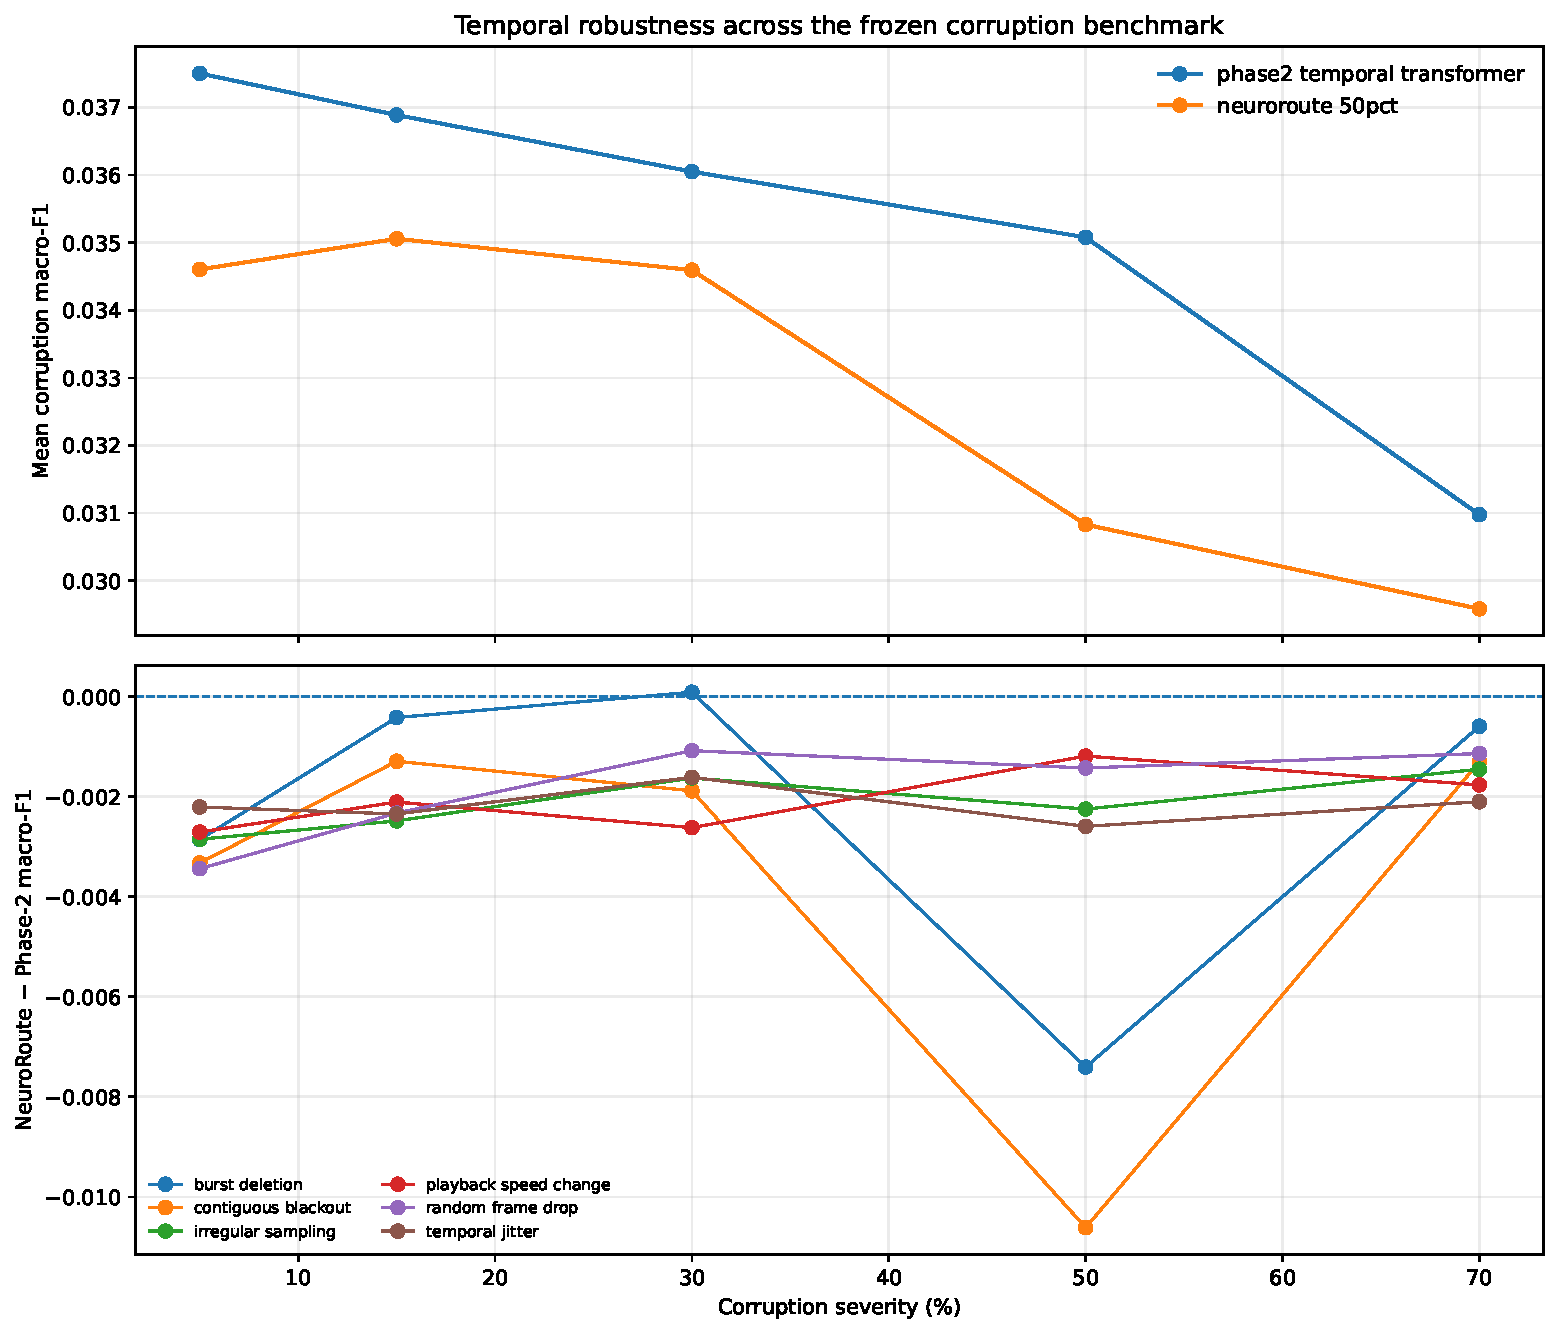
\includegraphics[width=0.94\linewidth]{figures/fig06_temporal_robustness.pdf}
\caption{Temporal-corruption robustness of the dense reference and the 50\% routed deployment. The routed model does not improve the average corruption macro-F1 under the frozen protocol.}
\label{fig:robustness}
\end{figure}

\subsection{Negative controls and EEG-free deployment}

The completed control study includes random EEG, wrong-subject EEG, temporally shifted EEG, and removal of meaningful neural supervision. Their clean macro-F1 values do not reveal a consistent neural-specific advantage over the no-neural baseline (Table~\ref{tab:controls}). This is consistent with the teacher diagnostics: the current neural representation is weak, so a strong causal benefit from EEG supervision should not be assumed.

The deployment audit provides a separate engineering result. The final visual-only artifact records \texttt{eeg\_required=false}, \texttt{eeg\_preprocessing\_required=false}, and \texttt{eeg\_encoder\_required=false}. Thus, the trained system can be serialized and executed without carrying the neural branch into inference. Figure~\ref{fig:controls} summarizes the control and deployment outcomes.

{\small\begin{table}[t]
\centering
\caption{Neural negative controls and EEG-free deployment audit.}
\label{tab:controls}
\begin{tabular}{lrl}
\toprule
Condition & Clean macro-F1 & Meaningful neural supervision \\
\midrule
Phase-2 dense visual & 0.0376 & No \\
NeuroRoute 50\textbackslash{}% & 0.0348 & Yes (training) \\
random eeg & 0.0370 & Control \\
wrong subject eeg & 0.0353 & Control \\
shifted eeg & 0.0344 & Control \\
no neural supervision & 0.0401 & Control \\
Deployment requirement & EEG-free & No EEG preprocessing / encoder \\
\bottomrule
\end{tabular}
\par\smallskip\noindent\footnotesize\textit{Note.} The completed NeuroRoute gate was INCONCLUSIVE: compute reduction and EEG-free deployment were established, whereas recognition preservation, robustness improvement, and a control-dependent neural effect were not.
\end{table}
}

\begin{figure}[t]
\centering
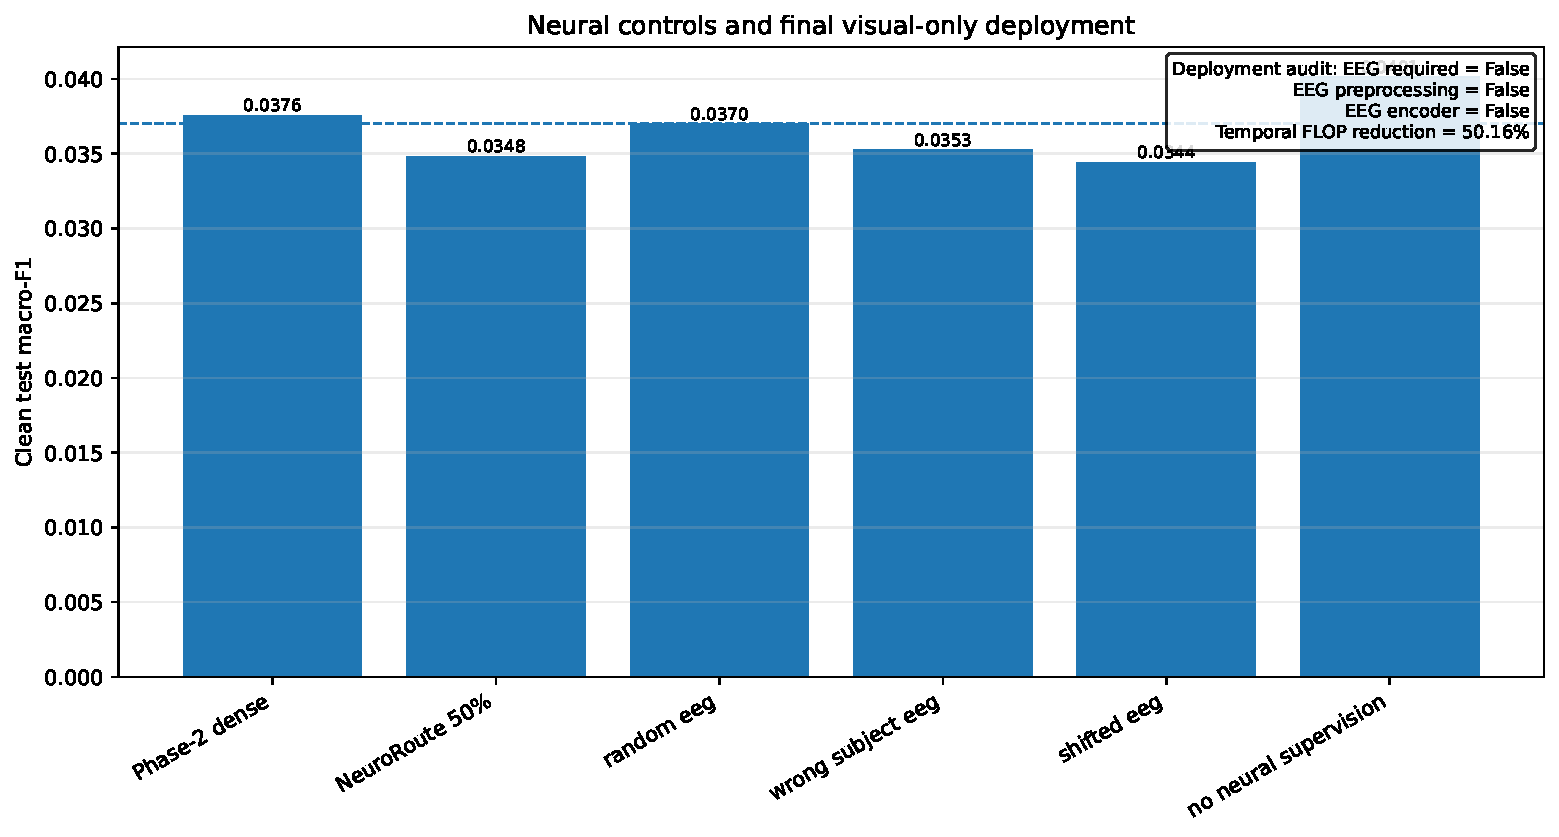
\includegraphics[width=0.92\linewidth]{figures/fig07_controls_and_deployment.pdf}
\caption{Negative controls and deployment audit. The deployment path is video-only, while the completed control experiments do not establish a neural-specific recognition advantage.}
\label{fig:controls}
\end{figure}

\subsection{Overall evidence status}

Taken together, the experiments establish four properties of the completed study: (i) a frozen synchronized and subject-independent benchmark, (ii) weak but measurable action-discriminative information in the standalone EEG teacher, (iii) approximately 50.16\% reduction in estimated temporal computation at the predefined 50\% budget, and (iv) an EEG-free deployed inference path. At the same time, three stronger claims are not established: recognition preservation, corruption-robustness improvement, and a statistically supported neural-specific subject-level gain. The final routing gate is therefore classified as \textsc{Inconclusive} rather than successful.

% =============================================================================
\section{Discussion}
% =============================================================================

\subsection{What the results establish}

The first contribution is methodological. The synchronization and leakage controls turn a naturally multimodal dataset into a reproducible subject-independent temporal-learning benchmark. This matters because training a complex multimodal network on a misaligned or subject-leaking index could produce artificially strong results that do not survive controlled evaluation.

The second contribution is diagnostic. The EEG teacher is not treated as automatically trustworthy privileged information. Its test macro-F1 is only slightly above the $1/27$ reference, while temporal shuffling produces a small change and importance remains close to uniform. These results indicate that the extracted EEG representation contains limited task-relevant structure at the temporal granularity used here. This finding is consistent with the broader challenge of subject variability and signal quality in EEG-based learning, and it cautions against assuming that synchronized neural data are necessarily informative for every downstream visual objective.

The third contribution is computational. Adaptive routing can halve the estimated temporal FLOPs without carrying EEG into deployment. This establishes the feasibility of the asymmetric training/deployment design as an engineering mechanism, even though it does not establish recognition preservation in the present experiment.

\subsection{Why neural supervision did not translate into a recognition gain}

Several explanations remain plausible and should be interpreted as hypotheses rather than demonstrated causes. First, the extracted 128-dimensional EEG representation may compress away temporal information that is useful for the action classes. Second, action labels derived from long real-world task intervals may not align tightly with the short neural dynamics represented by the one-second features. Third, subject variability may weaken cross-participant transfer of a neural representation. Finally, the visual and neural streams need not prioritize the same temporal evidence: a neural response can be discriminative for a human observer without identifying the precise visual tokens that a classifier needs for recognition.

The diagnostics support this uncertainty. The near-uniform importance distribution and very small shuffle effect suggest that a routing signal derived directly from the current teacher should not be expected to behave like a sharply peaked frame selector. In other words, the bottleneck may lie not in the routing mechanism itself but in the quality and task alignment of its supervisory source.

\subsection{Relation to prior work}

The distinction from prior EEG--video work is therefore functional rather than merely multimodal. EgoBrain established synchronized EEG--vision action understanding and Brain-TIM uses both modalities for multimodal prediction~\cite{lin2026egobrain}. Cavazza et al. demonstrated EEG as privileged information for training a video model that can operate without EEG at inference~\cite{cavazza2022actions}. Our study places the auxiliary neural information at a different point in the pipeline: the goal is to influence \emph{temporal allocation of visual computation}. This direction is also consistent with the broader literature on adaptive token/frame selection, but adds a neural supervisory source to the routing problem~\cite{ryoo2021tokenlearner,rao2021dynamicvit,wang2022adafocusv2,fu2025framefusion,li2026adaptok}.

\subsection{Implications for future neural priors}

The results suggest a useful design principle for multimodal learning: privileged modalities should be evaluated as signals with measurable reliability rather than assumed to be universally beneficial. For a neural prior to guide adaptive visual inference successfully, future systems may need more expressive temporal EEG representations, uncertainty-aware weighting of the teacher signal, finer temporal alignment, or supervision objectives that explicitly model delays between stimulus, neural response, and visually discriminative evidence. Such extensions should be evaluated under the same subject-independent controls rather than inferred from multimodal training loss alone.

% =============================================================================
\section{Limitations}
% =============================================================================

Several limitations define the scope of the present conclusions. First, the absolute recognition performance on the locked 27-class subject-independent task is low, so the routing result should be interpreted as an efficiency study rather than as a competitive action-recognition benchmark with state-of-the-art accuracy. Second, the EEG teacher provides only weak evidence of temporal structure in the current 128-dimensional representation; therefore, the present study does not establish that EEG is a strong neural temporal prior. Third, the adaptive route does not preserve clean recognition or mean corruption robustness in the completed experiment, and the final gate is accordingly inconclusive. Fourth, the main model operates on precomputed feature sequences rather than raw video frames, so the measured FLOP reduction is a temporal-backbone estimate rather than a full end-to-end reduction including feature extraction. Fifth, the primary frozen benchmark does not provide an explicit cross-scene metadata partition suitable for the same controlled evaluation, so cross-scene claims are outside the scope of the reported results. Finally, the temporal context is limited to eight one-second tokens, which constrains the kinds of long-range temporal routing behavior that can be observed.

% =============================================================================
\section{Conclusion}
% =============================================================================

This work presented a controlled investigation of neural-temporal supervision for adaptive egocentric video computation. Using a rigorously synchronized, subject-independent EgoBrain benchmark, we established a fixed evaluation protocol and independently characterized the information content of the extracted EEG representation. The EEG teacher was only weakly discriminative and exhibited limited temporal-order and importance concentration, while the completed adaptive-routing system reduced estimated temporal computation by 50.16\% at the predefined 50\% budget and required no EEG at deployment. At the same time, the routed model did not preserve the dense visual reference's recognition performance or improve temporal-corruption robustness, and the final scientific gate therefore remains inconclusive. The principal result is consequently not a claim that EEG-guided routing already solves efficient action recognition, but a reproducible framework that exposes both the computational potential and the current limits of neural privileged supervision for adaptive visual inference.

% =============================================================================
\begin{credits}
\subsubsection{\ackname}
The authors acknowledge the open availability of the EgoBrain dataset and software resources that enabled the present study.

\subsubsection{\discintname}
The authors have no competing interests to declare that are relevant to the content of this article.
\end{credits}

% =============================================================================
% References
% =============================================================================
\begin{thebibliography}{19}

\bibitem{lin2026egobrain}
Lin, N., Wang, Y., Han, D., Jiang, W.-B., Li, J., Furuta, R., Sato, Y., Li, D.:
EgoBrain: Synergizing Minds and Eyes For Human Action Understanding.
In: International Conference on Learning Representations (ICLR) (2026).

\bibitem{damen2022epickitchens}
Damen, D., Doughty, H., Farinella, G.M., Furnari, A., Kazakos, E., Ma, J., Moltisanti, D., Munro, J., Perrett, T., Price, W., Wray, M.:
Rescaling Egocentric Vision: Collection, Pipeline and Challenges for EPIC-KITCHENS-100.
International Journal of Computer Vision \textbf{130}, 33--55 (2022).

\bibitem{grauman2022ego4d}
Grauman, K., Westbury, A., Byrne, E., Chavis, Z., Furnari, A., Girdhar, R., et al.:
Ego4D: Around the World in 3,000 Hours of Egocentric Video.
In: Proceedings of the IEEE/CVF Conference on Computer Vision and Pattern Recognition (CVPR), pp. 18995--19012 (2022).

\bibitem{bertasius2021timesformer}
Bertasius, G., Wang, H., Torresani, L.:
Is Space-Time Attention All You Need for Video Understanding?
In: Proceedings of the 38th International Conference on Machine Learning (ICML), PMLR 139, pp. 813--824 (2021).

\bibitem{arnab2021vivit}
Arnab, A., Dehghani, M., Heigold, G., Sun, C., Lu\v{c}i\'c, M., Schmid, C.:
ViViT: A Video Vision Transformer.
In: Proceedings of the IEEE/CVF International Conference on Computer Vision (ICCV), pp. 6836--6846 (2021).

\bibitem{tong2022videomae}
Tong, Z., Song, Y., Wang, J., Wang, L.:
VideoMAE: Masked Autoencoders are Data-Efficient Learners for Self-Supervised Video Pre-Training.
In: Advances in Neural Information Processing Systems 35 (NeurIPS) (2022).

\bibitem{cavazza2022actions}
Cavazza, J., Ahmed, W., Volpi, R., Morerio, P., Bossi, F., Willemse, C., Wykowska, A., Murino, V.:
Understanding action concepts from videos and brain activity through subjects' consensus.
Scientific Reports \textbf{12}, 19073 (2022).

\bibitem{vapnik2009privileged}
Vapnik, V., Vashist, A.:
A new learning paradigm: Learning using privileged information.
Neural Networks \textbf{22}(5--6), 544--557 (2009).

\bibitem{hinton2015distillation}
Hinton, G., Vinyals, O., Dean, J.:
Distilling the Knowledge in a Neural Network.
In: NIPS Deep Learning and Representation Learning Workshop (2015).

\bibitem{wang2021adafocus}
Wang, Y., Chen, Z., Jiang, H., Song, S., Han, Y., Huang, G.:
Adaptive Focus for Efficient Video Recognition.
In: Proceedings of the IEEE/CVF International Conference on Computer Vision (ICCV), pp. 16249--16258 (2021).

\bibitem{ghodrati2021frameexit}
Ghodrati, A., Bejnordi, B.E., Habibian, A.:
FrameExit: Conditional Early Exiting for Efficient Video Recognition.
In: Proceedings of the IEEE/CVF Conference on Computer Vision and Pattern Recognition (CVPR), pp. 15608--15618 (2021).

\bibitem{ryoo2021tokenlearner}
Ryoo, M.S., Piergiovanni, A.J., Arnab, A., Dehghani, M., Angelova, A.:
TokenLearner: What Can 8 Learned Tokens Do for Images and Videos?
In: Advances in Neural Information Processing Systems 34 (NeurIPS) (2021).

\bibitem{rao2021dynamicvit}
Rao, Y., Zhao, W., Liu, B., Lu, J., Zhou, J., Hsieh, C.-J.:
DynamicViT: Efficient Vision Transformers with Dynamic Token Sparsification.
In: Advances in Neural Information Processing Systems 34 (NeurIPS) (2021).

\bibitem{wang2022adafocusv2}
Wang, Y., Yue, Y., Lin, Y., Jiang, H., Lai, Z., Kulikov, V., Orlov, N., Shi, H., Huang, G.:
AdaFocus V2: End-to-End Training of Spatial Dynamic Networks for Video Recognition.
In: Proceedings of the IEEE/CVF Conference on Computer Vision and Pattern Recognition (CVPR), pp. 20062--20072 (2022).

\bibitem{chalk2024tim}
Chalk, J., Huh, J., Kazakos, E., Zisserman, A., Damen, D.:
TIM: A Time Interval Machine for Audio-Visual Action Recognition.
In: Proceedings of the IEEE/CVF Conference on Computer Vision and Pattern Recognition (CVPR), pp. 18153--18163 (2024).

\bibitem{zeng2024temporalrobustness}
Zeng, R., Chen, X., Liang, J., Wu, H., Cao, G., Guo, Y.:
Benchmarking the Robustness of Temporal Action Detection Models Against Temporal Corruptions.
In: Proceedings of the IEEE/CVF Conference on Computer Vision and Pattern Recognition (CVPR), pp. 18263--18274 (2024).

\bibitem{fu2025framefusion}
Fu, T., Liu, T., Han, Q., Dai, G., Yan, S., Yang, H., Ning, X., Wang, Y.:
FrameFusion: Combining Similarity and Importance for Video Token Reduction on Large Vision Language Models.
In: Proceedings of the IEEE/CVF International Conference on Computer Vision (ICCV), pp. 22654--22663 (2025).

\bibitem{li2026adaptok}
Li, Y., Tian, C., Xia, R., Liao, N., Guo, W., Li, H., Dai, J., Li, H., Yang, X.:
AdapTok: Learning Adaptive and Temporally Causal Video Tokenization in a 1D Latent Space.
In: Proceedings of the IEEE/CVF Conference on Computer Vision and Pattern Recognition (CVPR), pp. 16163--16172 (2026).

\bibitem{jiang2024labram}
Jiang, W.-B., Zhao, L.-M., Lu, B.-L.:
Large Brain Model for Learning Generic Representations with Tremendous EEG Data in BCI.
In: International Conference on Learning Representations (ICLR) (2024).

\end{thebibliography}

\end{document}
